\chapter{Exigences}
Pour commencer cette partie d'étalement des exigences, qui est la suite de l'analyse des besoins de notre système. nous allons établir une liste d'exigences que doit respecter notre Robot Planteur. Vous y trouverez ensuite une Tables des exigences qui reprend la liste dans un diagramme spécifiques : un diagramme d'exigence. Enfin, nous allons lier les exigences obtenu dans les premières sous parties avec l'analyse des besoins des parties prenantes.

\section{Table des exigences}
\begin{figure}[!ht]
\centering
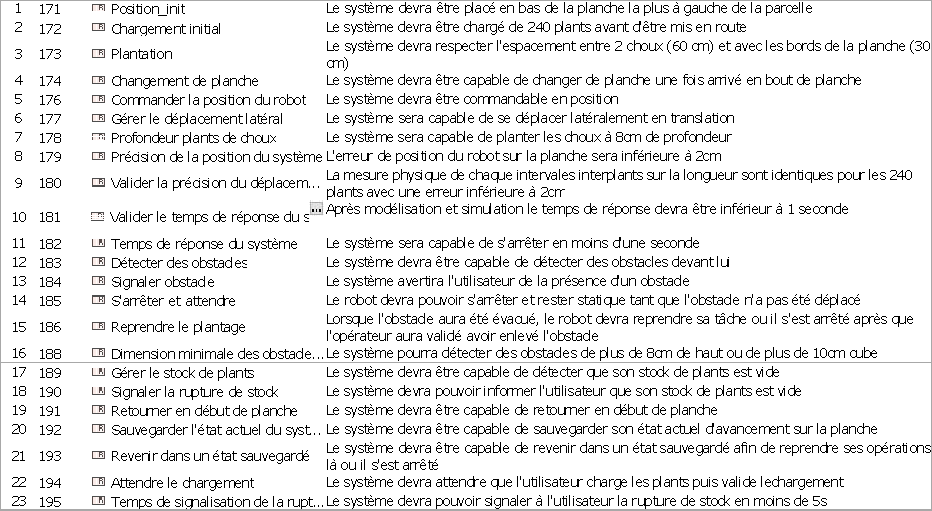
\includegraphics[width = .8\textwidth]{./II/images/SysML_Requirements_Table__Specifications_MOE__Specifications.pdf}
\caption{Table des exigences}\label{fig:requirementsTable}
\end{figure}

\section{Diagrammes des exigences}
Ce diagramme fait directement référence à la table des exigences. Nous avonschoisi de séparer les spécifications en 4 sous groupe qui sont
\begin{itemize}
\item [\textbullet] Spécifications non fonctionnelles 
\item [\textbullet]Spécifications fonctionnelles
\item [\textbullet] Spécifications de performance
\item [\textbullet] Spécifications de validation
\end{itemize}
\begin{figure}[!ht]
\centering
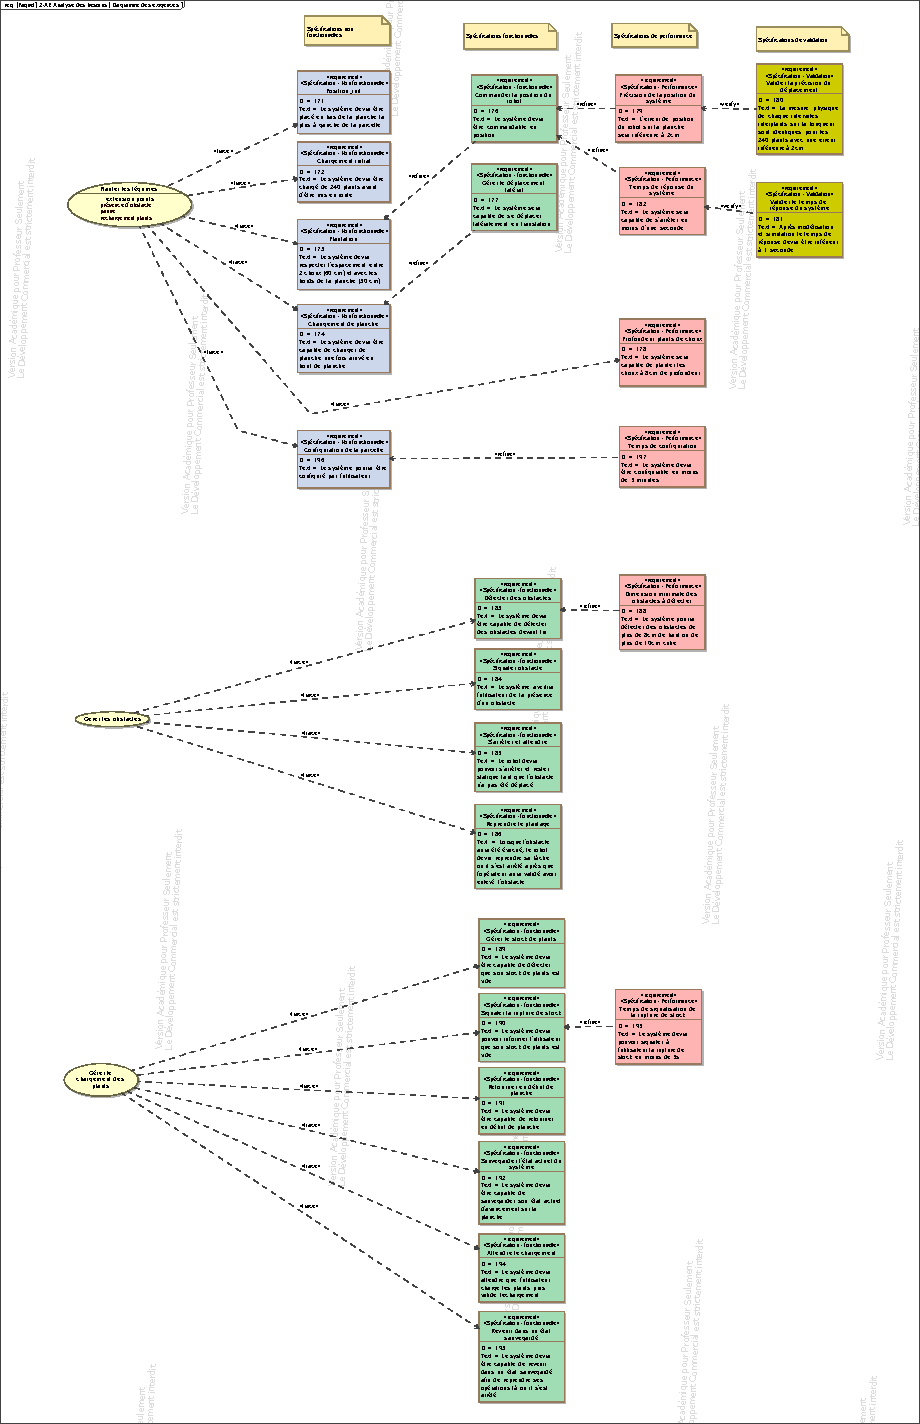
\includegraphics[width = .8\textwidth]{./II/images/SysML_Requirements_Diagram__2-AE_Analyse_des_besoins__Diagramme_des_exigences.pdf}
\caption{Diagramme des exigences}\label{fig:requirementsDiagram}
\end{figure}
\newpage

\section{Matrice de traçabilité}
Sur la prochaine figure \ref{fig:maticeTracabilite}, nous avons renseigné le Matrice de traçabilité, qui vient lier les Besoins MOA avec l'analyse des besoins. Nous avons accentuer l'importance du besoin "Réaliser la mission élémentaire en autonomie" car il nous semble qu'il s'agit l d'un besoin rudimentaire du robot. 
\begin{figure}[!ht]
\centering
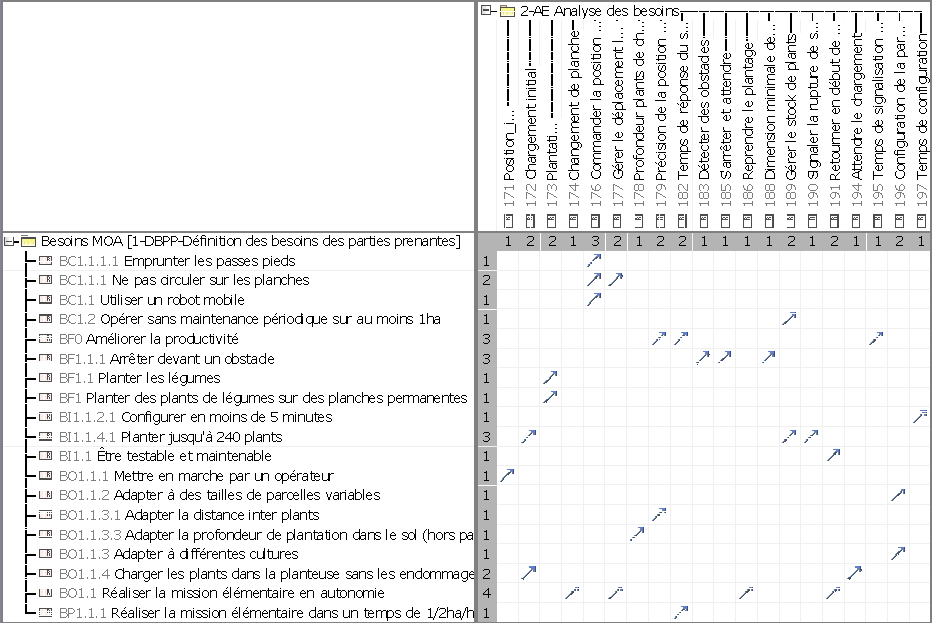
\includegraphics[width = \textwidth]{./II/images/Dependency_Matrix__2-AE_Analyse_des_besoins__Matrice_de_tracabilite.pdf}
\caption{Analyse des besoins Matrice de traçabilité}\label{fig:maticeTracabilite}
\end{figure}


